%%% LaTeX Template: Two column article
%%%
%%% Source: http://www.howtotex.com/
%%% Feel free to distribute this template, but please keep to referal to http://www.howtotex.com/ here.
%%% Date: February 2011

%%% Preamble
\documentclass[	DIV=calc,%
							paper=a4,%
							fontsize=12pt,%
							onecolumn]{scrartcl}	 					% KOMA-article class

\usepackage{lipsum}													% Package to create dummy text
\usepackage[brazil]{babel}										% English language/hyphenation
\usepackage[protrusion=true,expansion=true]{microtype}				% Better typography
\usepackage{amsmath,amsfonts,amsthm}					% Math packages
\usepackage[pdftex]{graphicx}									% Enable pdflatex
\usepackage[svgnames]{xcolor}									% Enabling colors by their 'svgnames'
\usepackage[hang, small,labelfont=bf,up,textfont=it,up]{caption}	% Custom captions under/above floats
\usepackage{epstopdf}												% Converts .eps to .pdf
\usepackage{subfig}													% Subfigures
\usepackage{booktabs}												% Nicer tables
\usepackage{fix-cm}													% Custom fontsizes
\usepackage{float}
\usepackage[utf8]{inputenc}
\usepackage[top=2.5cm, bottom=2.5cm, left=2.5cm, right=2.5cm]{geometry}
\usepackage[ddmmyyyy]{datetime}
\addto\captionsenglish{%
	\renewcommand\tablename{Tabela}
	\renewcommand\figurename{Figura}
} 
 

 
%%% Custom sectioning (sectsty package)
\usepackage{sectsty}													% Custom sectioning (see below)
\allsectionsfont{%															% Change font of al section commands
	\usefont{OT1}{phv}{b}{n}%										% bch-b-n: CharterBT-Bold font
	}

\sectionfont{%																% Change font of \section command
	\usefont{OT1}{phv}{b}{n}%										% bch-b-n: CharterBT-Bold font
	}



%%% Headers and footers
\usepackage{fancyhdr}												% Needed to define custom headers/footers
	\pagestyle{fancy}														% Enabling the custom headers/footers
\usepackage{lastpage}	

% Header (empty)
\lhead{}
\chead{}
\rhead{}
% Footer (you may change this to your own needs)

%% ====================================
%% ====================================
%% mude o rodape  do projeto
%% ====================================
%% ====================================

\lfoot{\footnotesize \texttt{Cabeamento estruturado} \textbullet ~Modelo de projeto}


\cfoot{}
\rfoot{\footnotesize página \thepage\ de \pageref{LastPage}}	% "Page 1 of 2"
\renewcommand{\headrulewidth}{0.0pt}
\renewcommand{\footrulewidth}{0.4pt}



%%% Creating an initial of the very first character of the content
\usepackage{lettrine}
\newcommand{\initial}[1]{%
     \lettrine[lines=3,lhang=0.3,nindent=0em]{
     				\color{DarkGoldenrod}
     				{\textsf{#1}}}{}}



%%% Title, author and date metadata
\usepackage{titling}															% For custom titles

\newcommand{\HorRule}{\color{DarkGoldenrod}%			% Creating a horizontal rule
									  	\rule{\linewidth}{1pt}%
										}

\pretitle{\vspace{-30pt} \begin{flushleft} \HorRule 
				\fontsize{50}{50} \usefont{OT1}{phv}{b}{n} \color{DarkRed} \selectfont 
				}

%% ====================================
%% ====================================
%% mude o titulo  do projeto
%% ====================================
%% ====================================

\title{Projeto de cabeamento estruturado}					% Title of your article goes here

%% ====================================



\posttitle{\par\end{flushleft}\vskip 0.5em}

\preauthor{\begin{flushleft}
					\large \lineskip 0.5em \usefont{OT1}{phv}{b}{sl} \color{DarkRed}}
\author{Antonio Domingos Isaias }  	% Author name goes here


\postauthor{\footnotesize \usefont{OT1}{phv}{m}{sl} \color{Black} 
	                \\Curso de Pós Graduação em Redes de Computadores
					\\Universidade Tecnológica Federal do Paraná - Câmpus Cornélio Procópio 								% Institution of author
					\par\end{flushleft}\HorRule}

\date{}																				% No date




%%% Begin document
\begin{document}
\maketitle
\thispagestyle{fancy} 	
\thispagestyle{empty}		% Enabling the custom headers/footers for the first page 
% The first character should be within \initial{}




%% ====================================
%% ====================================
%% mude o resumo  do projeto
%% ====================================
%% ====================================
\initial{E}\textbf{ste projeto tem o propósito de demonstrar a implantação de cabeamento estruturado em uma pequena empresa revendedora de veículos. A estrutura apresentada aqui é fictícia, entretanto, baseia-se em casos reais, pois demonstra um estrutura mínima necessária para atuar neste seguimento.
	Em projetos desta natureza é comum o cliente primeiro se preocupar com o layout do ambiente, portanto, após o arquiteto preparar a planta do ambiente, é necessário fazer uma planta da infrastrutura de dados que atenda este ambiente, e com esta determinar os materiais necessários, custos e fixa um prazo para conclusão da obra  
	.}

%% ====================================
\begin{figure}
	\centering
	\includegraphics{utfpr}
\end{figure}

\vspace{3cm}
\centerline{\textit{\textbf{\today}}}

\clearpage
    \renewcommand*\listfigurename{Lista de figuras}
\listoffigures

\renewcommand*\listtablename{Lista de tabelas}
\listoftables




\clearpage
\renewcommand{\contentsname}{Sumário}
\tableofcontents
\clearpage

%% ====================================
%% ====================================
%% Inicio do texto
%% ====================================
%% ====================================
\section{Introdução}
Instalação de infrastrutura de rede de computadores para atender a 10 pontos, sendo: 7 (sete) equipamentos desktop, 2 (dois) access point e 1 (uma) impressora multifuncional.
Preparação de rack para abrigar 1 servidor, 1 concentrador (switch) e 2 links de dados.


\subsection{Benefícios}
Criação de ramal exclusivo para cabeamento de dados, assim isolando os cabos de dados dos demais cabos existem no prédio, sem contar a facilidade em adicionar novos pontos, bastando lançado os cabos através das calhas perfiladas que serão instaladas. Haverá também dois roteadores wireless que proverá cobertura wi-fi por toda a área da empresa.

\subsection{Organizações Envolvidas}

\begin{table}[h!] % coloque h! para forcar a posicao
	\centering
	\label{my-label}
	\begin{tabular}{|l|l|l|}
		\hline
		\multicolumn{1}{|c|}{\textbf{INSTALAÇÃO}} & \multicolumn{1}{c|}{\textbf{EMPRESA}} & \multicolumn{1}{c|}{\textbf{RESPONSÁVEL}} \\ \hline
		Piso Elevado                              & L.A. Pisos                             & José Dias                                  \\ \hline
		Calhas Perfilada                              & Vitor Sales Elétrica                   & Marcos Roberto                             \\ \hline
		Cabeamento                                & Evolução Digital                       & Antonio Carlos                             \\ \hline
		Configuração do Rack                      & Evolução Digital                       & Antonio Carlos                             \\ \hline
		Acess Point                      & Evolução Digital                       & Antonio Carlos                             \\ \hline		
		Certificação                              & J.B. Net                               & João Batista                               \\ \hline
		Link 1 de 50Mbps                              & Vivo                               & -                                      \\ \hline
		Link 2 de 30Mbps                              & Net                              & -                               \\ \hline				
	\end{tabular}
\end{table}


\section{Estado atual}
Prédio em processo de reformado, sem infraestrutura de dados instalada anteriormente.

\section{Requisitos}
Devido a exigência de acesso a internet para aprovação de fichas de financiamento pelos bancos credenciados, é esperado máxima disponibilidade no acesso e redundância de link. 

\section{Usuários e Aplicativos}
Os usuários basicamente terão acesso a internet e ao sistema de ERP da empresa, a seção de contabilidade terá acesso à softwares contábeis e de folha de pagamento. O ERP da empresa e os softwares contábeis serão instalados no servidor e terão uma necessidade de garantia de disponibilidade média, entretanto, o acesso a internet a garantia de disponibilidade é alta.  Há um desejo dos responsáveis pela empresa em criar um departamento para vendas pela internet, entretanto, o local para instalação física ainda não foi definido.

\subsection{Usuários x Aplicativos}

\begin{table}[H] % coloque h! para forcar a posicao
		\caption{Usuários x aplicativos}
	\centering
	\begin{tabular}{|l|c|c|c|}
		\hline
		\multicolumn{1}{|c|}{\textbf{USUÁRIOS}} & \textbf{ERP DA EMPRESA} & \textbf{SOFT.CONTABEIS} & \textbf{INTERNET} \\ \hline
		Diretor                                 & X                       & X                       & X                 \\ \hline
		Gerente                                 & X                       & X                       & X                 \\ \hline
		Contabilidade                           & X                       & X                       & X                 \\ \hline
		Despachante Usuário 1                   & X                       &                         & X                 \\ \hline
		Despachante Usuário 2                   & X                       &                         & X                 \\ \hline
		Vendedor 1                              & X                       &                         & X                 \\ \hline
		Vendedor 2                              & X                       &                         & X                 \\ \hline
		Vendedor 3                              & X                       &                         & X                 \\ \hline
		Wi-fi                     &                        &                         & X                 \\ \hline		
	\end{tabular}
\end{table}


\section{Estrutura predial existente}

O prédio possui em sua parte térrea 16 mts de frente (largura), 5 mts do piso térreo ao piso superior (altura) e 14 mts de lado (comprimento). Na parte superior as medidas são 16 mts de largura, 6 mts de comprimento e 3 mts de altura.
Na parte térrea ficará o setor de vendas e a gerência, além do pátio de exposição dos veículos a venda. A ligação da parte térrea com a parte superior se dará por uma escada existente na extremidade do prédio.
A parte superior será composta pelas seções de Despachante, Contabilidade, Diretória e CPD.    

\begin{figure}[H]
	\centering
	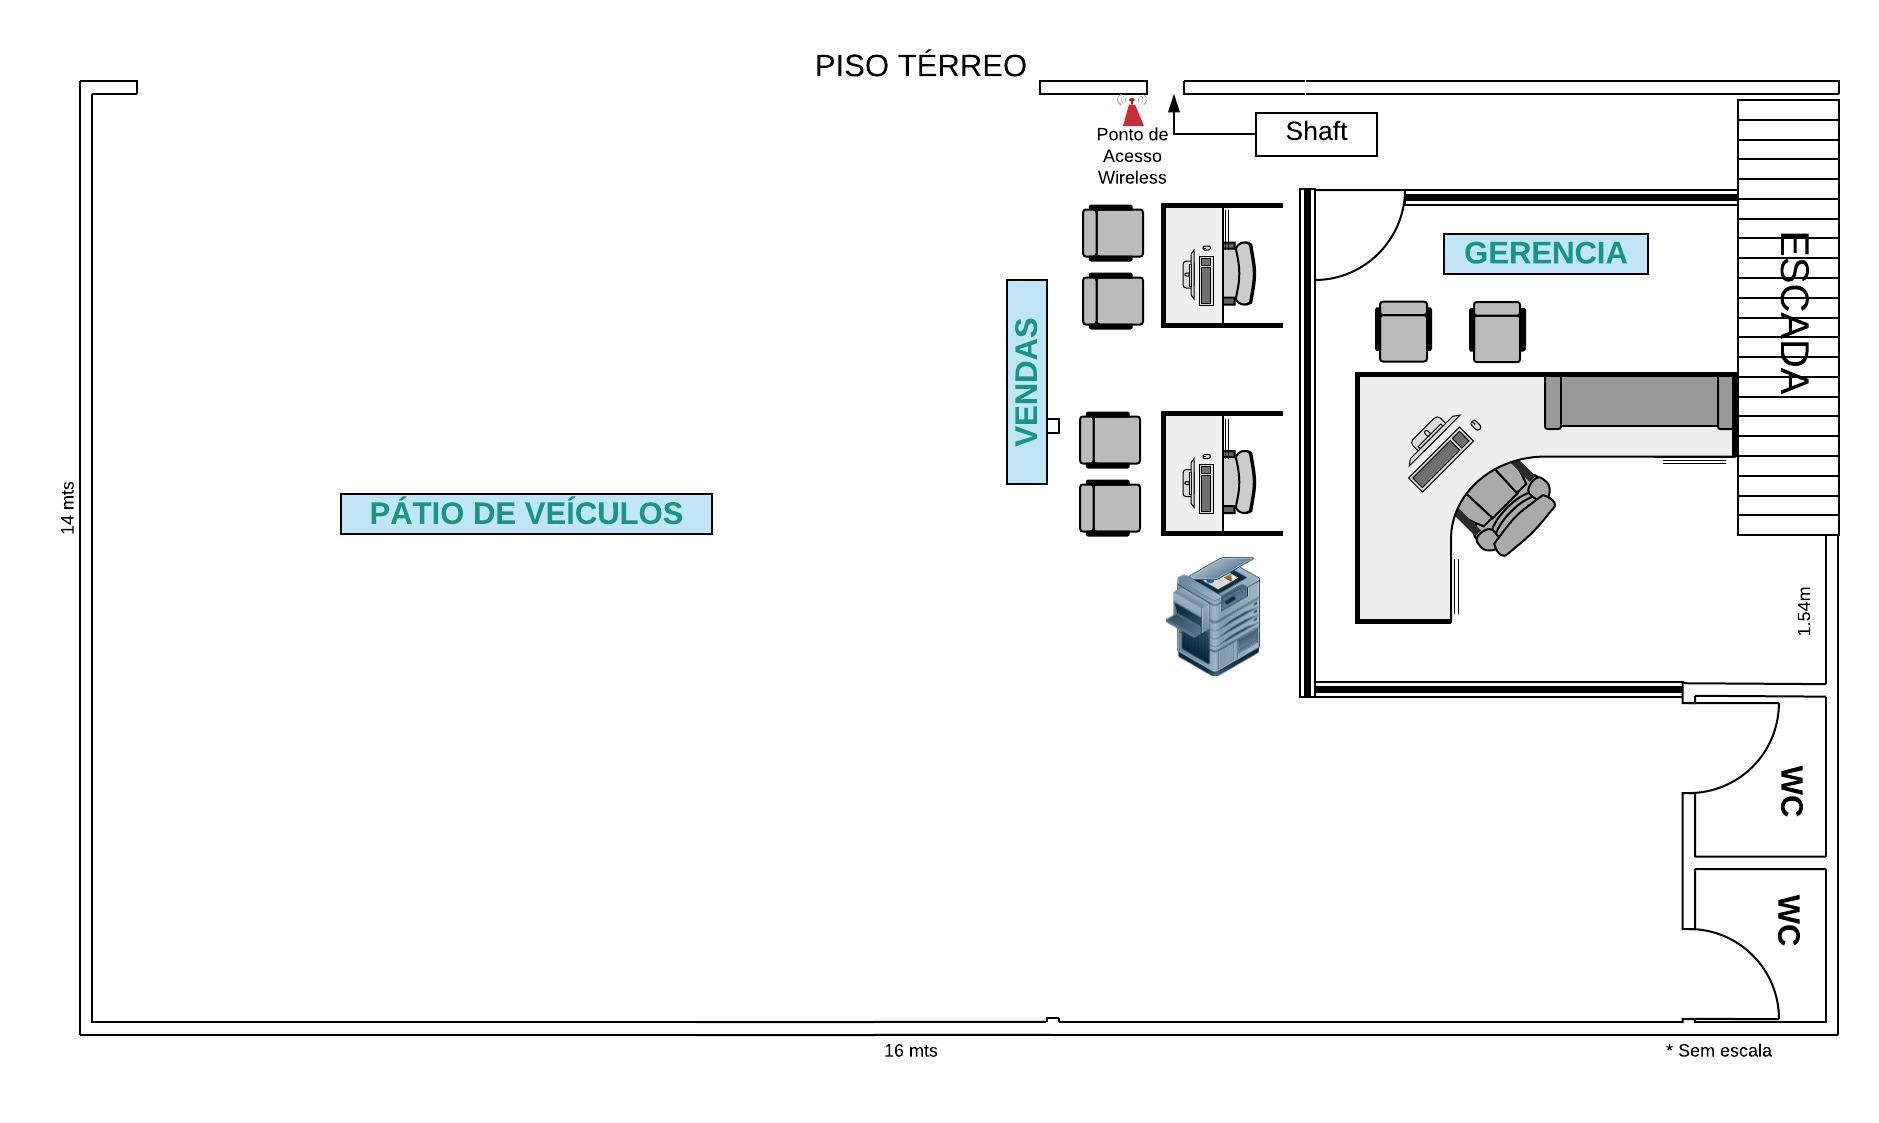
\includegraphics[width=\textwidth]{PlantadoAmbienteTerreo}
	\caption{Planta térrea do ambiente sem escala}
	\label{fig1}
\end{figure}

\begin{figure}[H]
	\centering
	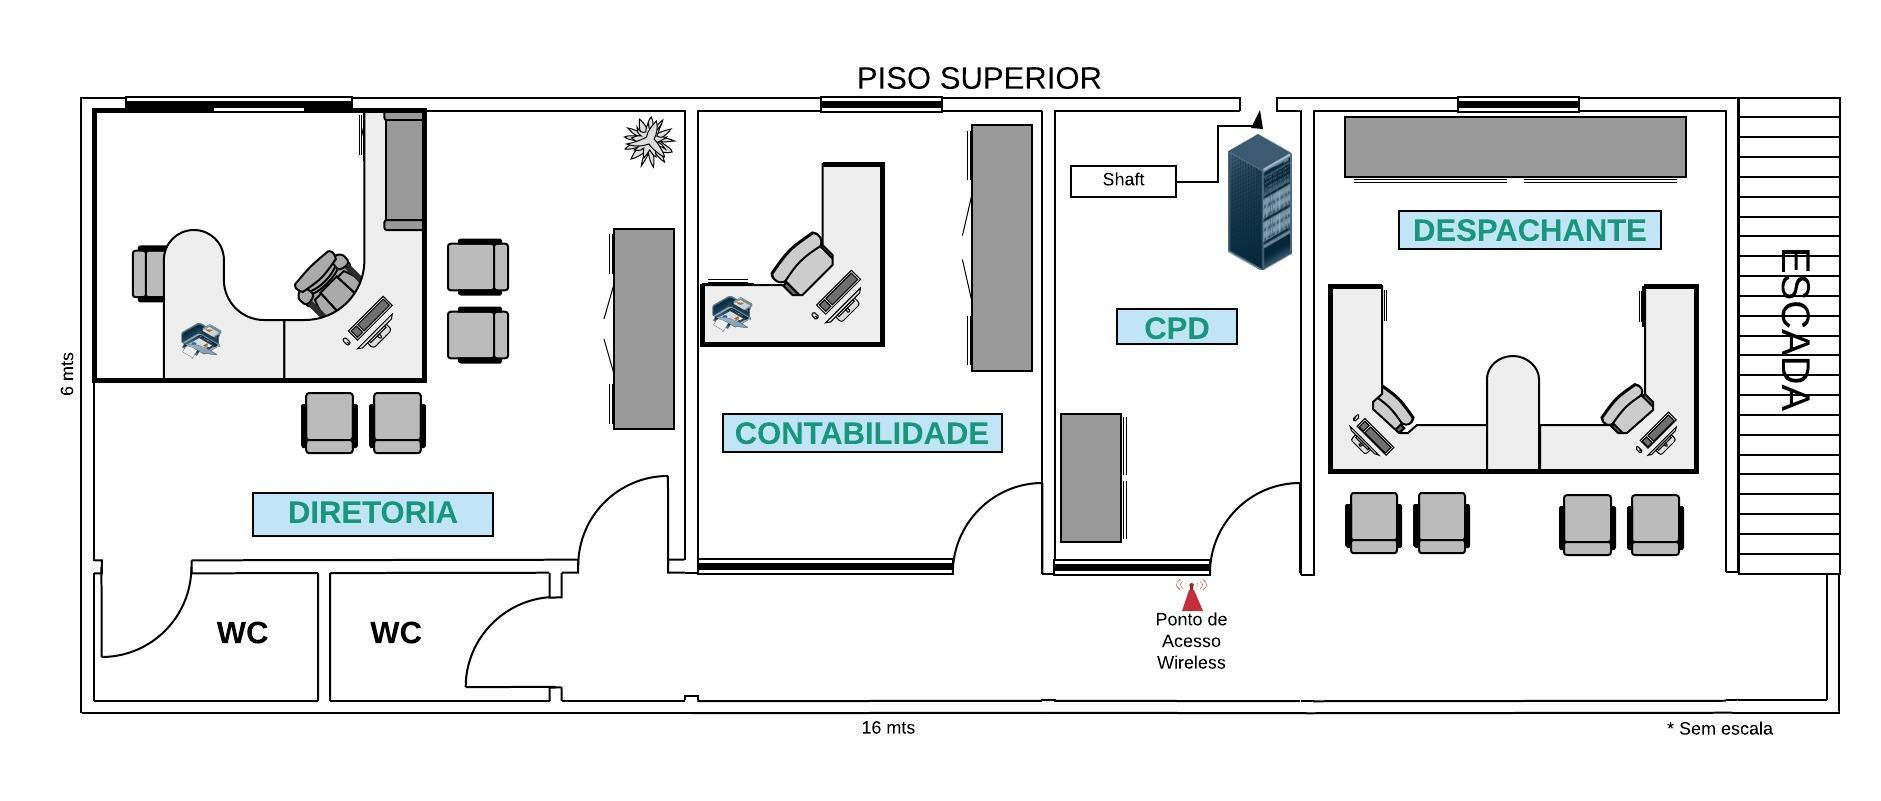
\includegraphics[width=\textwidth]{PlantadoAmbienteSuperior}
	\caption{Planta superior do ambiente sem escala}
	\label{fig2}
\end{figure}

\section{Planta Lógica - Elementos estruturados}

\subsection{Estado atual}
O prédio não possui infraestrutura de dados atualmente.

\subsection{Topologia}
Para atender as necessidades expostas no projeto apresentando na planta do ambiente Figura 1 e Figura 2, será necessário a instalação de piso elevado e calhas perfiladas para passagem dos campos de rede. 
O rack contendo o servidor de aplicação, switch, patch panel, roteadores dos dos links de internet ficarão na sala do CPD no piso superior.
Haverá dois access point, um no piso térreo e outro no piso superior, serão suficientes para cobrir toda área da empresa. Os APs propagarão dois SSID, um
com sufixo 'redeint' que dará acesso a rede lan e servidores e outro com sufixo 'cliente' que proverá somente acesso web ao clientes durante o período que estiverem na loja.

\begin{figure}[H]
	\centering
	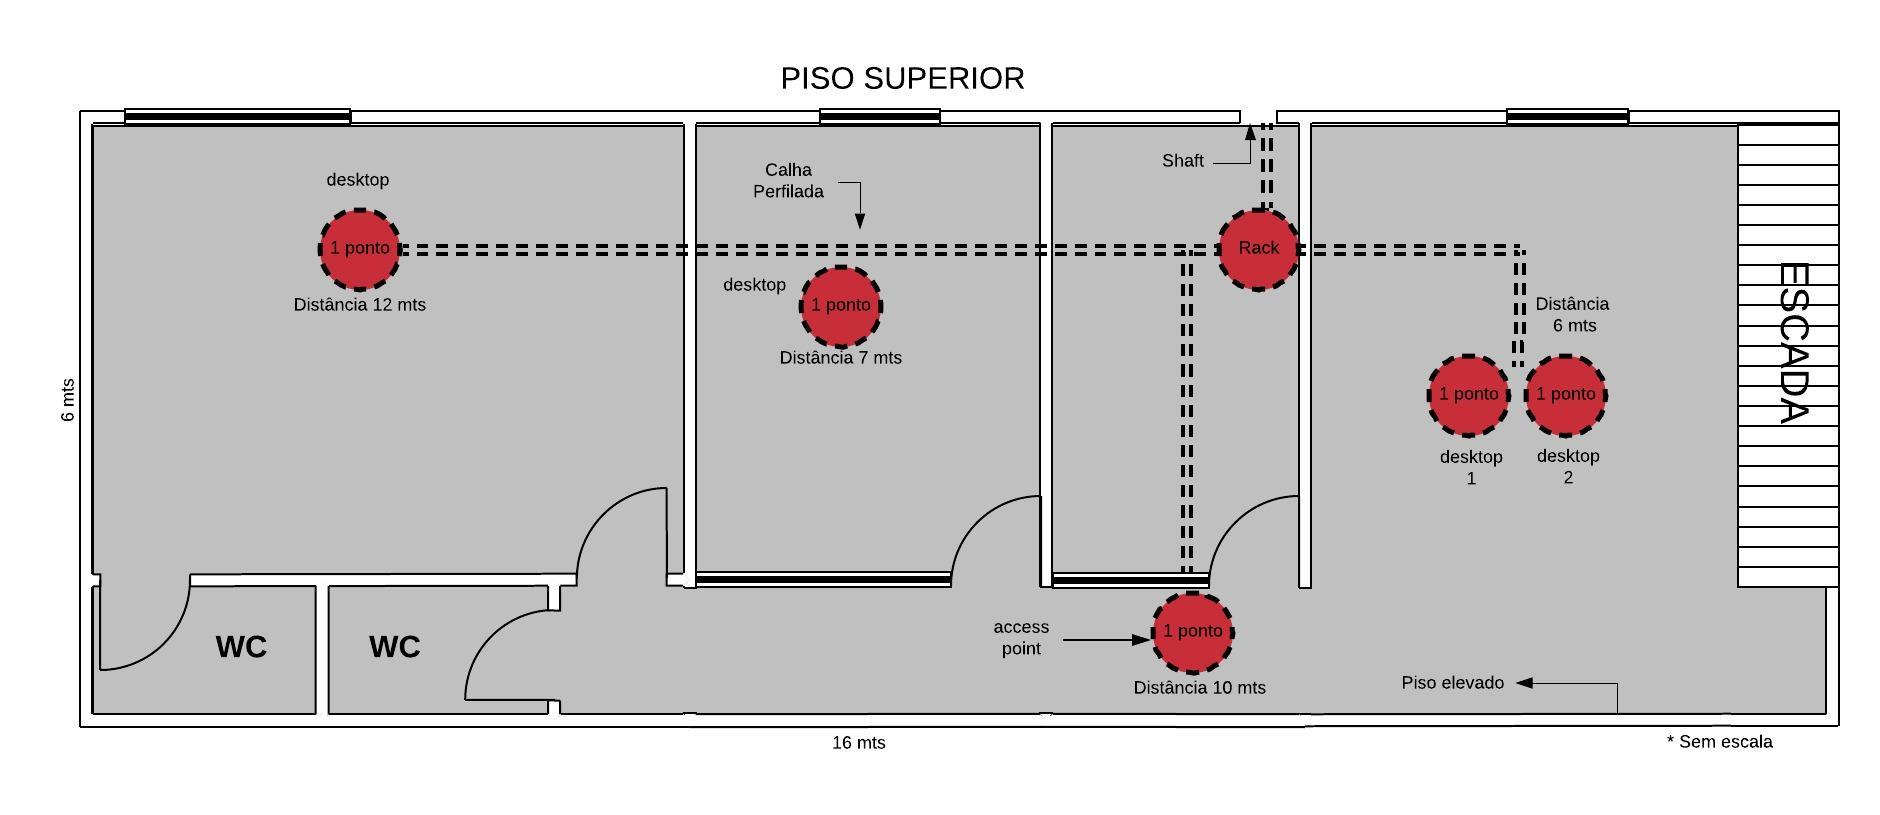
\includegraphics[width=\textwidth]{InfraestruturaSuperior}
	\caption{Planta da infraestrutura superior sem escala}
	\label{fig4}
\end{figure}

\begin{figure}[H]
	\centering
	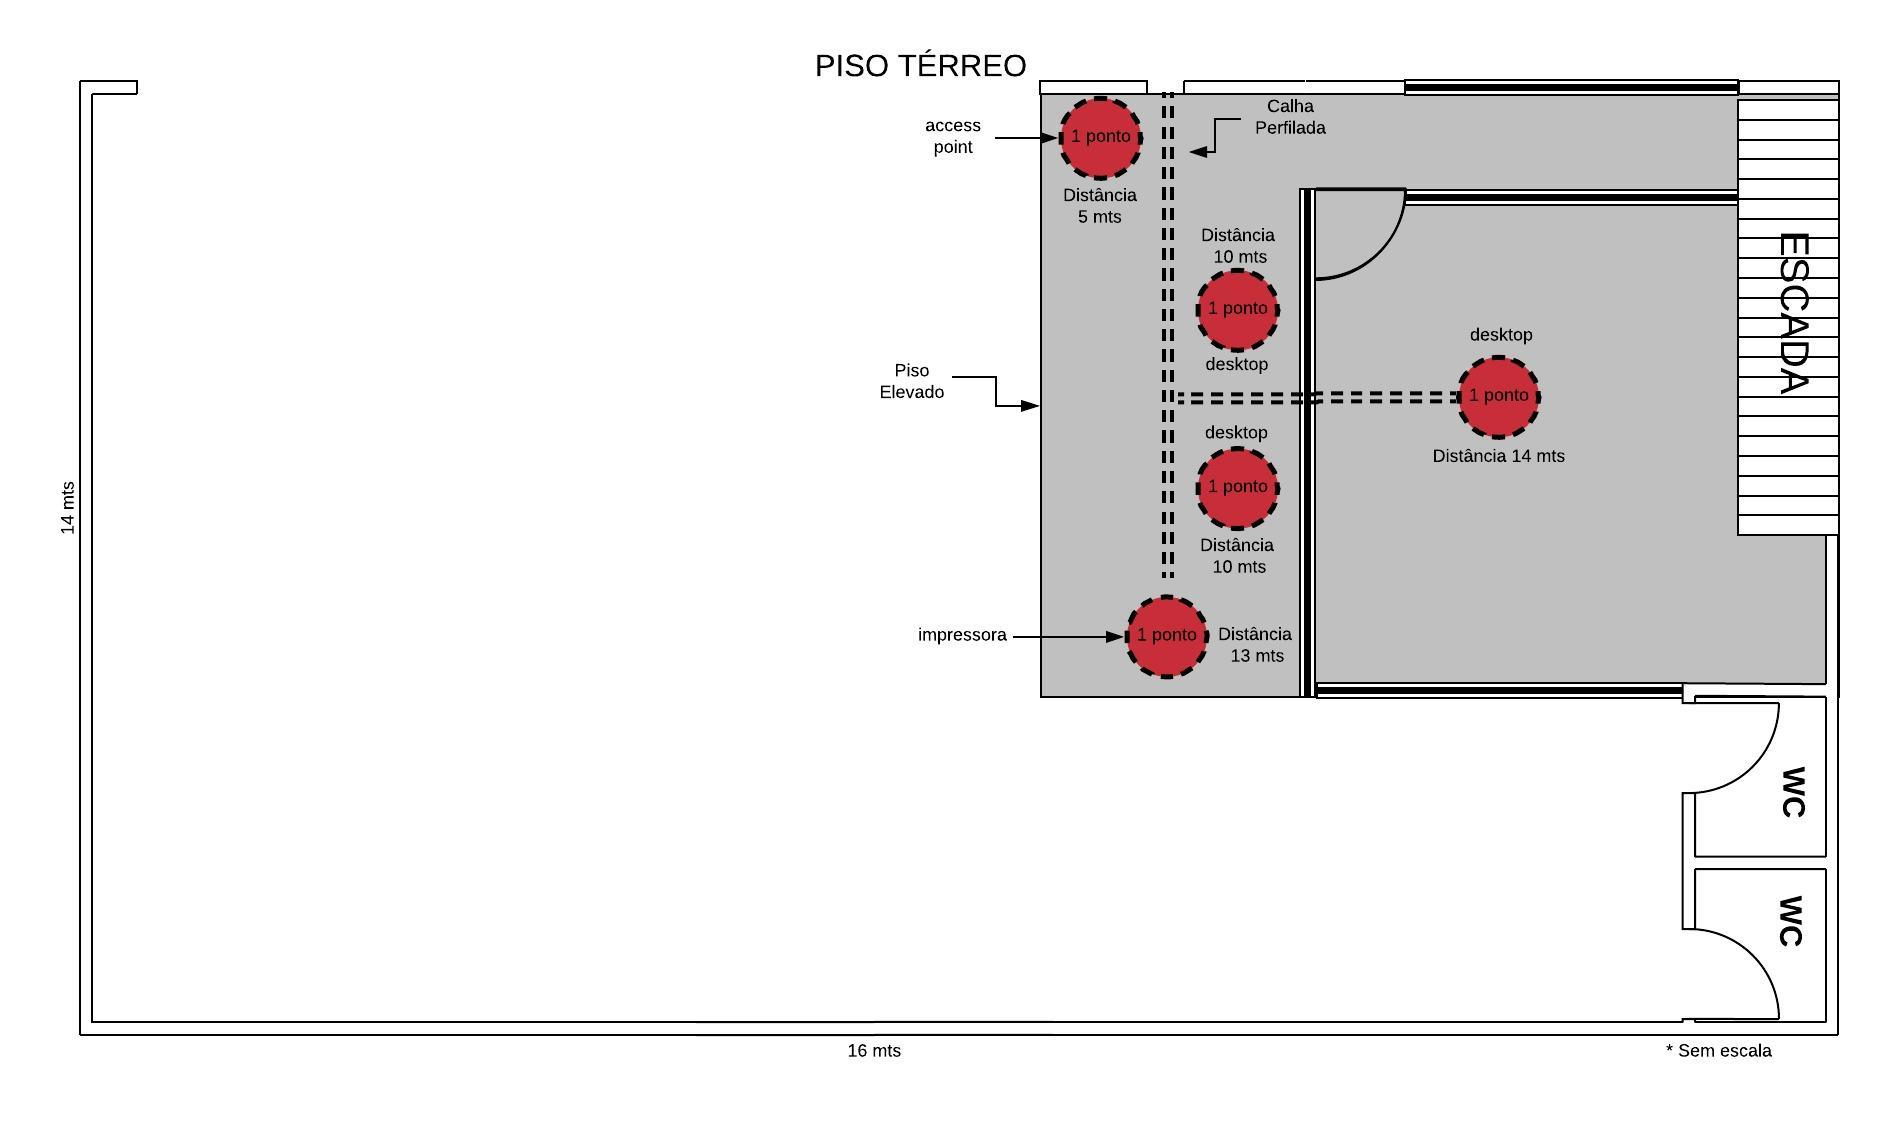
\includegraphics[width=\textwidth]{InfraestruturaTerreo}
	\caption{Planta da infraestrutura térrea sem escala}
	\label{fig3}
\end{figure}


\subsection{Encaminhamento}
Os cabos seguirão por calhas perfiladas sobre o piso elevado, e por calhas que interligarão o piso superior ao piso térreo. 

\subsection{Memorial descritivo}

\begin{table}[H]
	\centering
	\caption{Relação de passivos}
\label{my-label}
\begin{tabular}{|l|c|c|}
	\hline
	\multicolumn{1}{|c|}{\textbf{Passivos}}    & \textbf{Quantidade} & \textbf{Fabricante} \\ \hline
	Cabo UTP Cat5e                             & 93 mts              & Furukawa            \\ \hline
	Tomada RJ45 & 10 pçs               & Furukawa             \\ \hline
	Path Panel 24 portas Cat5e                 & 01 pç                & Furukawa            \\ \hline
	Path Cord Cat5e  2,5mts                    & 10 pçs               & Furukawa            \\ \hline
	Path Cord Cat5e  1,0mt                     & 12 pçs              & Furukawa            \\ \hline
	Régua de 12 tomadas para rack 19"          & 01 pç                & RCG                 \\ \hline
\end{tabular}
\end{table}

\subsection{Identificação dos cabos}
Os cabos serão identificados nas extremidades dos pontos, seguindo o seguinte padrão: XXY, onde XX representa a porta do patch panel e Y representa o andar onde será instalado o ponto, sendo A para o piso térreo e B para o piso superior.
A tabela 3 contem a relação de usuários e sua respectiva identificação para os pontos que já foram definidos, conforme plantas da Figura 3 e Figura 4. 

\begin{table}[H]
	\centering
	\caption{Tabela de identificação dos pontos}
	\label{my-label}
	\begin{tabular}{|l|c|c|c|}
		\hline
		\multicolumn{1}{|c|}{\textbf{USUÁRIOS}} & \multicolumn{1}{l|}{\textbf{Porta do Patch Panel}} & \multicolumn{1}{l|}{\textbf{Piso}} & \textbf{Identificação do Ponto} \\ \hline
		Servidor NIC 1                          & 01                                                 & B                                  & 01B                             \\ \hline
		Servidor NIC 2                          & 02                                                 & B                                  & 02B                             \\ \hline
		Diretor                                 & 03                                                 & B                                  & 03B                             \\ \hline
		Contabilidade                           & 04                                                 & B                                  & 04B                             \\ \hline
		Despachante Usuário 1                   & 05                                                 & B                                  & 05B                             \\ \hline
		Despachante Usuário 2                   & 06                                                 & B                                  & 06B                             \\ \hline
		Access Point Piso Superior              & 07                                                 & B                                  & 07B                             \\ \hline
		Gerência                                & 08                                                 & A                                  & 08A                             \\ \hline
		Vendedor 1                              & 09                                                 & A                                  & 09A                             \\ \hline
		Vendedor 2                              & 10                                                 & A                                  & 10A                             \\ \hline
		Impressora térreo                       & 11                                                 & A                                  & 11A                             \\ \hline
		Access Point Piso térreo                & 12                                                 & A                                  & 12A                             \\ \hline
	\end{tabular}
\end{table}

\section{Implantação}

\begin{figure}[H]
	\centering
	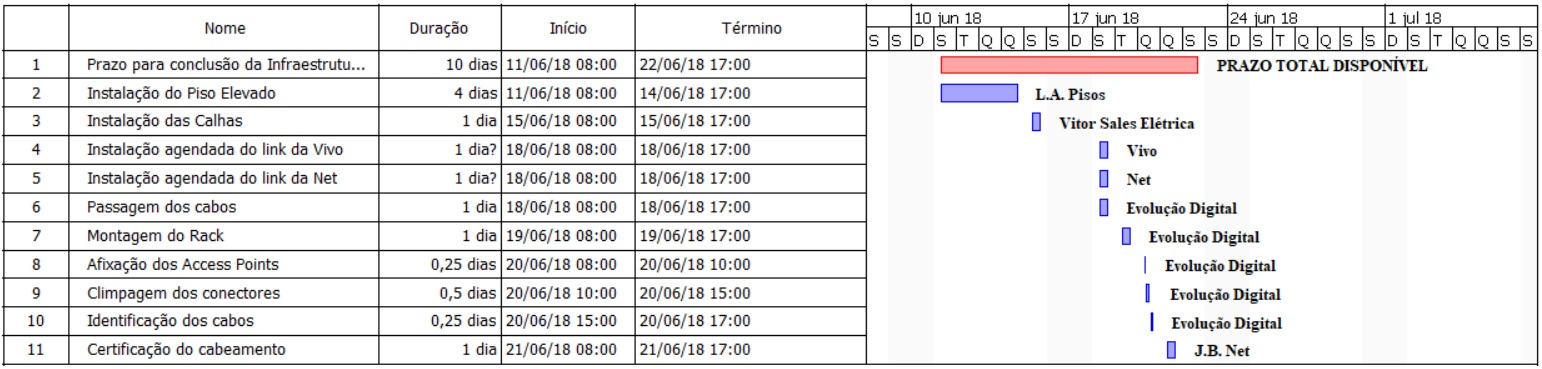
\includegraphics[width=\textwidth]{Cronograma}
	\caption{Cronograma de instalação}
	\label{fig5}
\end{figure}

\section{Plano de certificação}
A certificação será executada antes da abertura oficial da loja (inauguração), tendo em vista deixar o ambiente pronto para uso já no primeiro dia útil de trabalho da empresa. A serviço de certificação visará detecta falhas na instalação dos passivos, identificar interferências externa nos cabos, problemas com conectores ou patch panel.
Como comprimento máximo do cabo do ponto mais extremo é de 15 metros, não é esperado problema de atenuação quanto a distância.
Os testes serão realizados do keystone (tomada RJ) do ponto do cliente até o patch panel, os patch cords não necessitarão ser certificados, pois já serão adquiridos de fabrica com esta característica.
Os testes serão realizados conforme padrão TIA 568-C.2 e, após aprovação de todos os pontos, será emitido relatório detalhado de Wire Map, atenuação, Capacitância, Resistência, NEXT/FEXT, Perda de Retorno e outros parâmetros sobre a eficiência dos passivos testados. Tais relatórios deverão ser arquivados em pasta própria para consultas futuras se houver necessidade.

\section{Plano de manutenção}
A cada período de 6 (seis) meses é recomendado a inspeção visual na estação física dos equipamento a procura de focos de infiltração de água, vestígios de roedores ou outros fatores que poderão interferir na qualidade da infraestrutura. 


\subsection{Plano de expansão}
A estrutura atual de camada 2 possibilita a expansão de mais 12 pontos de rede sem necessidade de troca de equipamentos instalados.

\section{Risco}
Atraso na instalação ou indisponibilidade de links de dados por parte das operadoras de telefonia.

\section{Orçamento}

\begin{table}[H]
	\centering
	\caption{Custos do Projeto}
	\label{my-label}
	\scalebox{0.7}{
	\begin{tabular}{lrcrrll}
		\hline
		\multicolumn{1}{|c|}{\textbf{Material / Serviço}}          & \multicolumn{1}{c|}{\textbf{Qtde}} & \multicolumn{1}{c|}{\textbf{Unid}} & \multicolumn{1}{c|}{\textbf{V. Unitário}} & \multicolumn{1}{c|}{\textbf{V. Total}} & \multicolumn{1}{c|}{\textbf{Marca}} & \multicolumn{1}{c|}{\textbf{Fornecedor}}  \\ \hline
		\multicolumn{1}{|l|}{Tomada RJ45}                          & \multicolumn{1}{r|}{17}            & \multicolumn{1}{c|}{pç}            & \multicolumn{1}{r|}{R\$ 11,00}            & \multicolumn{1}{r|}{R\$ 187,00}        & \multicolumn{1}{l|}{Furukawa}       & \multicolumn{1}{l|}{Evolução Digital}     \\ \hline
		\multicolumn{1}{|l|}{Cabos de rede}                        & \multicolumn{1}{r|}{93}            & \multicolumn{1}{c|}{mt}            & \multicolumn{1}{r|}{R\$ 2,50}             & \multicolumn{1}{r|}{R\$ 232,50}        & \multicolumn{1}{l|}{Furukawa}       & \multicolumn{1}{l|}{Evolução Digital}     \\ \hline
		\multicolumn{1}{|l|}{Switch 24 Portas Giga Sg1024d 19"}    & \multicolumn{1}{r|}{1}             & \multicolumn{1}{c|}{pç}            & \multicolumn{1}{r|}{R\$ 470,00}           & \multicolumn{1}{r|}{R\$ 470,00}        & \multicolumn{1}{l|}{Tp-link}        & \multicolumn{1}{l|}{Evolução Digital}     \\ \hline
		\multicolumn{1}{|l|}{Path Panel 24 portas Cat.5e}          & \multicolumn{1}{r|}{1}             & \multicolumn{1}{c|}{pç}            & \multicolumn{1}{r|}{R\$ 185,00}           & \multicolumn{1}{r|}{R\$ 185,00}        & \multicolumn{1}{l|}{Furukawa}       & \multicolumn{1}{l|}{Evolução Digital}     \\ \hline
		\multicolumn{1}{|l|}{Path Cord Cat.5e 2,5 mts}             & \multicolumn{1}{r|}{10}            & \multicolumn{1}{c|}{pç}            & \multicolumn{1}{r|}{R\$ 17,00}            & \multicolumn{1}{r|}{R\$ 170,00}        & \multicolumn{1}{l|}{Furukawa}       & \multicolumn{1}{l|}{Evolução Digital}     \\ \hline
		\multicolumn{1}{|l|}{Path Cord Cat.5e 1,0 mts}             & \multicolumn{1}{r|}{12}            & \multicolumn{1}{c|}{pç}            & \multicolumn{1}{r|}{R\$ 7,30}             & \multicolumn{1}{r|}{R\$ 87,60}         & \multicolumn{1}{l|}{Furukawa}       & \multicolumn{1}{l|}{Evolução Digital}     \\ \hline
		\multicolumn{1}{|l|}{Regua de 12 tomada para rack 19"}     & \multicolumn{1}{r|}{1}             & \multicolumn{1}{c|}{pç}            & \multicolumn{1}{r|}{R\$ 29,00}            & \multicolumn{1}{r|}{R\$ 29,00}         & \multicolumn{1}{l|}{RCG}            & \multicolumn{1}{l|}{WBX Racks}            \\ \hline
		\multicolumn{1}{|l|}{Access Point 4p Linksys E2500}        & \multicolumn{1}{r|}{2}             & \multicolumn{1}{c|}{pç}            & \multicolumn{1}{r|}{R\$ 263,00}           & \multicolumn{1}{r|}{R\$ 526,00}        & \multicolumn{1}{l|}{Linksys}        & \multicolumn{1}{l|}{Evolução Digital}     \\ \hline
		\multicolumn{1}{|l|}{Rack Piso Fechado 20U x 670mm}        & \multicolumn{1}{r|}{1}             & \multicolumn{1}{c|}{pç}            & \multicolumn{1}{r|}{R\$ 918,00}           & \multicolumn{1}{r|}{R\$ 918,00}        & \multicolumn{1}{l|}{WBX Racks}      & \multicolumn{1}{l|}{WBX Racks}            \\ \hline
		\multicolumn{1}{|l|}{Kit de Exaustor p/ Rack – 4 ventil.}  & \multicolumn{1}{r|}{1}             & \multicolumn{1}{c|}{kit}           & \multicolumn{1}{r|}{R\$ 356,00}           & \multicolumn{1}{r|}{R\$ 356,00}        & \multicolumn{1}{l|}{WBX Racks}      & \multicolumn{1}{l|}{WBX Racks}            \\ \hline
		\multicolumn{1}{|l|}{Bandeja Fixa Front. 2U x 290mm 19"}   & \multicolumn{1}{r|}{1}             & \multicolumn{1}{c|}{pç}            & \multicolumn{1}{r|}{R\$ 38,50}            & \multicolumn{1}{r|}{R\$ 38,50}         & \multicolumn{1}{l|}{WBX Racks}      & \multicolumn{1}{l|}{WBX Racks}            \\ \hline
		\multicolumn{1}{|l|}{Kit porca gaiola com 10 peças}        & \multicolumn{1}{r|}{5}             & \multicolumn{1}{c|}{kit}           & \multicolumn{1}{r|}{R\$ 6,70}             & \multicolumn{1}{r|}{R\$ 33,50}         & \multicolumn{1}{l|}{WBX Racks}      & \multicolumn{1}{l|}{WBX Racks}            \\ \hline
		\multicolumn{1}{|l|}{Guia de cabos 1U}                     & \multicolumn{1}{r|}{1}             & \multicolumn{1}{c|}{pç}            & \multicolumn{1}{r|}{R\$ 17,30}            & \multicolumn{1}{r|}{R\$ 17,30}         & \multicolumn{1}{l|}{WBX Racks}      & \multicolumn{1}{l|}{WBX Racks}            \\ \hline
		\multicolumn{1}{|l|}{Serviço de Passagens de Cabos}        & \multicolumn{1}{r|}{1}             & \multicolumn{1}{c|}{pç}            & \multicolumn{1}{r|}{R\$ 300,00}           & \multicolumn{1}{r|}{R\$ 300,00}        & \multicolumn{1}{c|}{-}              & \multicolumn{1}{l|}{Evolução Digital}     \\ \hline
		\multicolumn{1}{|l|}{Serviço de Montagem do Rack}          & \multicolumn{1}{r|}{1}             & \multicolumn{1}{c|}{pç}            & \multicolumn{1}{r|}{R\$ 120,00}           & \multicolumn{1}{r|}{R\$ 120,00}        & \multicolumn{1}{c|}{-}              & \multicolumn{1}{l|}{Evolução Digital}     \\ \hline
		\multicolumn{1}{|l|}{Serviço Climp. conectores e tomadas}  & \multicolumn{1}{r|}{10}            & \multicolumn{1}{c|}{pç}            & \multicolumn{1}{r|}{R\$ 15,00}            & \multicolumn{1}{r|}{R\$ 150,00}        & \multicolumn{1}{c|}{-}              & \multicolumn{1}{l|}{Evolução Digital}     \\ \hline
		\multicolumn{1}{|l|}{Serviço de Identificação de cabos}    & \multicolumn{1}{r|}{10}            & \multicolumn{1}{c|}{pç}            & \multicolumn{1}{r|}{R\$ 10,00}            & \multicolumn{1}{r|}{R\$ 100,00}        & \multicolumn{1}{c|}{-}              & \multicolumn{1}{l|}{Evolução Digital}     \\ \hline
		\multicolumn{1}{|l|}{Serviço de Afixação de Access Point}  & \multicolumn{1}{r|}{2}             & \multicolumn{1}{c|}{pç}            & \multicolumn{1}{r|}{R\$ 15,00}            & \multicolumn{1}{r|}{R\$ 30,00}         & \multicolumn{1}{c|}{-}              & \multicolumn{1}{l|}{Evolução Digital}     \\ \hline
		\multicolumn{1}{|l|}{Serviço de Certificação}              & \multicolumn{1}{r|}{10}            & \multicolumn{1}{c|}{pç}            & \multicolumn{1}{r|}{R\$ 50,00}            & \multicolumn{1}{r|}{R\$ 500,00}        & \multicolumn{1}{c|}{-}              & \multicolumn{1}{l|}{J.B Net}              \\ \hline
		\multicolumn{1}{|l|}{Inst. piso elevado + 8 Cx de tomada*} & \multicolumn{1}{r|}{145}           & \multicolumn{1}{c|}{mt}            & \multicolumn{1}{r|}{R\$ 120,00}           & \multicolumn{1}{r|}{R\$ 17.400,00}     & \multicolumn{1}{c|}{-}              & \multicolumn{1}{l|}{L.A. Pisos}           \\ \hline
		\multicolumn{1}{|l|}{Instalação das calhas perfilhadas *}  & \multicolumn{1}{r|}{40}            & \multicolumn{1}{c|}{mt}            & \multicolumn{1}{r|}{R\$ 35,00}            & \multicolumn{1}{r|}{R\$ 1.400,00}      & \multicolumn{1}{c|}{-}              & \multicolumn{1}{l|}{Vitor Sales Elétrica} \\ \hline
		\multicolumn{4}{l}{\textbf{TOTAL GERAL DOS CUSTOS}}                                                                                                                              & \textbf{R\$ 23.250,40}                 & \multicolumn{2}{l}{}                                                            \\ \hline
		\** Incluso material e mão de obra
	\end{tabular}}
\end{table}


\section{Recomendações}
Em caso de manutenção sobre o piso elevado será necessário acompanhar a intervenção para garantir que não haverá modificações inadvertidas na rede de dados ou uso das calhas para outros fins que poderão causar interferências e consequentemente problemas instabilidade na rede.
Quando da instalação de novo ponto, este deverá ser realizado por pessoal qualificado observado o plano de certificação e tabela de identificação dos pontos (ver Tabela 3).

\section{Referências bibliográficas}
https://tex.stackexchange.com/questions/10863/is-there-a-way-to-slightly-shrink-a-table-including-font-size-to-fit-within-th/10864


https://nuvem.utfpr.edu.br/index.php/s/6xb5XpeCwKIFvpr


https://docente.ifrn.edu.br/tadeuferreira/disciplinas/2013.2/cabeamento-estruturado/A12.pdf


http://blog.samuelcavalcante.com/wp-content/uploads/2010/12/03-Aula-de-Cabeamento-04-Identificadores.pdf


https://www.youtube.com/watch?v=23sdpkoD3yU 

*******************************************************

\end{document}